\subsection{Missing transverse energy}

Many interesting physics processes are with the involvement of neutrinos.
Since they do not interact with any materials in the detector, neutrinos cannot be detected directly;
but instead, they can result in imbalance in the plane transverse to the beam axis, where momentum conservation is assumed.
It is known as the missing transverse momentum denoted as $E_{T}^{miss}$,
which is obtained from the negative vector sum of the momenta of all particles detected in a proton-proton collision event.

The $E_{T}^{miss}$ is measured using selected, reconstructed and calibrated hard objects in an event.
Its x- and y- components can be calculated as follow\cite{Aaboud2018}:
\begin{equation} \label{eq:met_xy}
	E_{x(y)}^{miss} = E_{x(y)}^{miss, e} + E_{x(y)}^{miss, \gamma} + E_{x(y)}^{miss, \tau} + E_{x(y)}^{miss, jets} + E_{x(y)}^{miss, \mu} + E_{x(y)}^{miss, soft}
\end{equation}
where each object term is given by the negative vectorial sum of the momenta of the respective calibrated objects.
The calorimeter signals are associated with the reconstructed objects in the following order: electrons, photons, hadronically decaying taus, jets, muons.
The soft term is reconstructed from detected objects not match any hard object passing the selections, but associated with the primary vertex.
Details of applied selections for each term are summarized in table~\ref{tab:met_sele}.
\begin{table}[!htbp]
  \begin{center}
  \small
  \caption{Overview of the contributions to $E_{T}^{miss}$.}
  \label{tab:met_sele}
  \begin{tabular}{p{1cm}p{1.5cm}p{5cm}p{1.5cm}p{5cm}}
    \toprule
     \multicolumn{5}{c}{Objects contributing to $E_{T}^{miss}$} \\
     \hline
     Priority & Type & Selections & Variables & Comments \\
     \hline
     (1) & $e$          & $|\eta|<1.37~or~1.52<|\eta|<2.47 \newline p_{T}>10 GeV$ & $E_{T}^{miss, e}$      
         & all $e^{\pm}$ passing kinematic selections and medium reconstruction quality \\ 
     \hline
     (2) & $\gamma$     & $|\eta|<1.37~or~1.52<|\eta|<2.47 \newline p_{T}>25 GeV$ & $E_{T}^{miss, \gamma}$ 
         & all $\gamma$ passing kinematic selections and tight reconstruction quality, and without overlapping with (1) \\
     \hline
     (3) & $\tau_{had}$ & $|\eta|<1.37~or~1.52<|\eta|<2.47 \newline p_{T}>20 GeV$ & $E_{T}^{miss, \tau}$   
         & all $\tau_{had}$ passing kinematic selections and medium reconstruction quality, and without overlapping with (1) and (2) \\
     \hline
     (4) & $\mu$        & $|\eta|<2.7 \newline p_{T}>10 GeV$ & $E_{T}^{miss, \mu}$
         & all $\mu$ passing kinematic selections and medium reconstruction quality \\
     \hline
     (5) & jet          & $|\eta|<4.5 \newline p_{T}>60 GeV \newline 
			--- or --- \newline 
			2.4<|\eta|<4.5 \newline 20 GeV<p_{T}<60 GeV \newline
			--- or --- \newline
			|\eta|<2.4 \newline 20 GeV<p_{T}<60 GeV \newline JVT>0.59$ & $E_{T}^{miss, jet}$
         & all jets passing kinematic selections and reconstruction quality (jet cleaning) , and without overlap with (1)–(4) \\
     \hline
     (6) & ID track     & $p_{T}>400 MeV \newline 
			|d_{0}|<1.5 mm \newline 
			|z_{0}sin\theta|<1.5 mm \newline 
			\Delta R(track, e/\gamma cluster)>0.05 \newline 
			\Delta R(track, \tau_{had})> 0.2$       &  $E_{T}^{miss, soft}$ 
         & all ID tracks from the hard-scattering vertex passing kinematic selections and reconstruction quality, and not associated with any particle from (1), (3) or (4), or associated with a jet from (5) \\
    \bottomrule
  \end{tabular}
  \end{center}
\end{table}

Based on $E_{x(y)}^{miss}$, the magnitude of $E_{T}^{miss}$ and the azimuthal angle $\phi^{miss}$ are computed:
\begin{equation}
\begin{split}
	E_{T}^{miss} &= \sqrt{ \left(E_{x}^{miss}\right)^{2} + \left(E_{y}^{miss}\right)^{2} } \\
	\phi^{miss} &= arctan \left(E_{y}^{miss}/E_{x}^{miss}\right)
\end{split}
\end{equation}

In equation~\ref{eq:met_xy}, each objects are required to pass certain reconstruction and calibrated criteria and selections mentioned above before taken as inputs.

In figure~\ref{fig:met_dis}, left plot shows the observed $E_{T}^{miss}$ distribution for data and MC of $Z \rightarrow \mu\mu$ events that without genuine missing transverse momentum;
and right plot shows the $E_{T}^{miss}$ distribution for $W \rightarrow e\nu$ events that has genuine (true) missing transverse momentum due to real neutrino.
\begin{figure}[!htb]
  \centering
  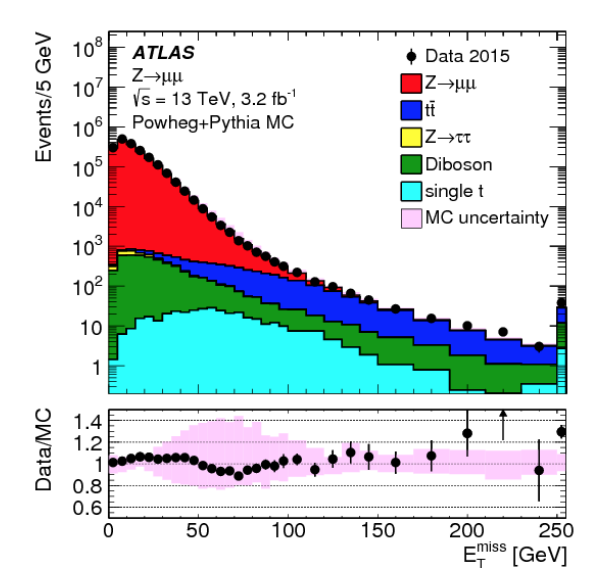
\includegraphics[width=0.42\textwidth]{figures/Simulation/met_Zmm.png}
  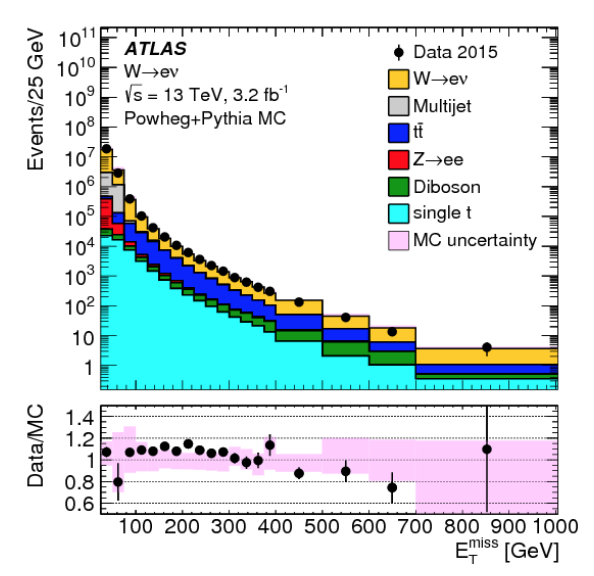
\includegraphics[width=0.42\textwidth]{figures/Simulation/met_Wev.png}
  \caption{Measured $E_{T}^{miss}$ distribution for $Z \rightarrow \mu\mu$ events (left) and $W \rightarrow e\nu$ events (right). }
  \label{fig:met_dis}
\end{figure}
